\chapter{Image-based steganography}

In this chapter we will cover the term steganography and explain 
how can we measure its strength. Then we will proceed to image-based
(specifically to JPEG-based) steganography. We will end this chapter
with overview of present state in free and/or open-source software
for steganography on Android platform.

\section{What steganography is?}

Steganography is an art of hiding information. The difference between steganography and
cryptography is that the goal of cryptography is to hide the content of message, whereas
the goal of steganography is to conceal the very fact that the message exists.

\subsubsection{A bit of terminology}

Information, which we want to hide, is often called \textit{secret message}. The object,
in which we want to embed our secret message, is often called \textit{cover message} (or, in our case,
\textit{cover image}). Additional information, required to detect and extract the secret message
from cover object, is called \textit{stegokey} (as opposed to cryptokey, which is used to 
unveil the content of the message). If the stegokey, needed to embed a message is different
from the key, needed to extract it, we call this steganographic method \textit{asymmetric}. In
other case, we call it \textit{symmetric}.

\subsubsection{How to measure strength of steganographic methods?}

Basic idea is simple: if a message concealed by method X was not discovered, then it's a good method.
But the concealing power depends on the message length (analogy: it is relatively easy
to write one date on your schooldesk without having your professor seeing it, but it's a lot
harder to write a whole textbook on it). 

Keeping that in mind, one can never tell with $100\%$
guarantee that this object doesn't carry any message, as sometimes it could carry only a few bits.

As for embedded messages are often encrypted and the order of bits is permuted, it is hard
to actually extract the message. So it is reasonable only talk about the possibility to
distinguish between ''clean'' images and images with hidden messages. 

\section{Image-based steganography}
\label{sec:image-steganography}

How to hide messages in lossless image formats and why it isn't a good idea.

\TODO lossless images stego and discussion about suitability

\section{JPEG compression algorithm}
\label{sec:jpeg}

JPEG format provides many options for storing images. We will talk about
one of the most common versions. For further details we recommend to read \TODO source.

Input of compression algorithm is a raw image with pixels encoded
in RGB model (each pixel is encoded as three 8-bit numbers, representing
red, green and blue component of resulting colour, resluting in 24 bits of information
per pixel).

Compression consists of several steps:
\begin{enumerate}
    \item Transformation from RGB to YCbCr color space
    \item Reduction of Cb and Cr channels definition (lossy operation)
    \item Splitting each channel into $8 \times 8$ bytes long blocks 
    \item Discrete cosine transformation (DCT) of numbers in each block
    \item Rounding of DCT coefficients (main lossy operation)
    \item (Lossless) compression of coefficients (main compression operation)
\end{enumerate}

\subsubsection{Color space transformation}

Pixels are transformed from RGB to YCbCr color space. Y channel represents
brightness of a pixel ({which can be viewed as greyscale copy of the original image}),
Cb and Cr components represent so called \textit{chrominance} -- color without brightness. 
You can see example in figure \ref{img:YCbCr}.


%(based on source: \url{https://en.wikipedia.org/wiki/File:Barns_grand_tetons_YCbCr_separation.jpg})
\begin{figure}
%vlozenie samotneho obrazku vycentrovaneho a vhodnej velkosti
%obrazok je v subore images/cervik.png
\centerline{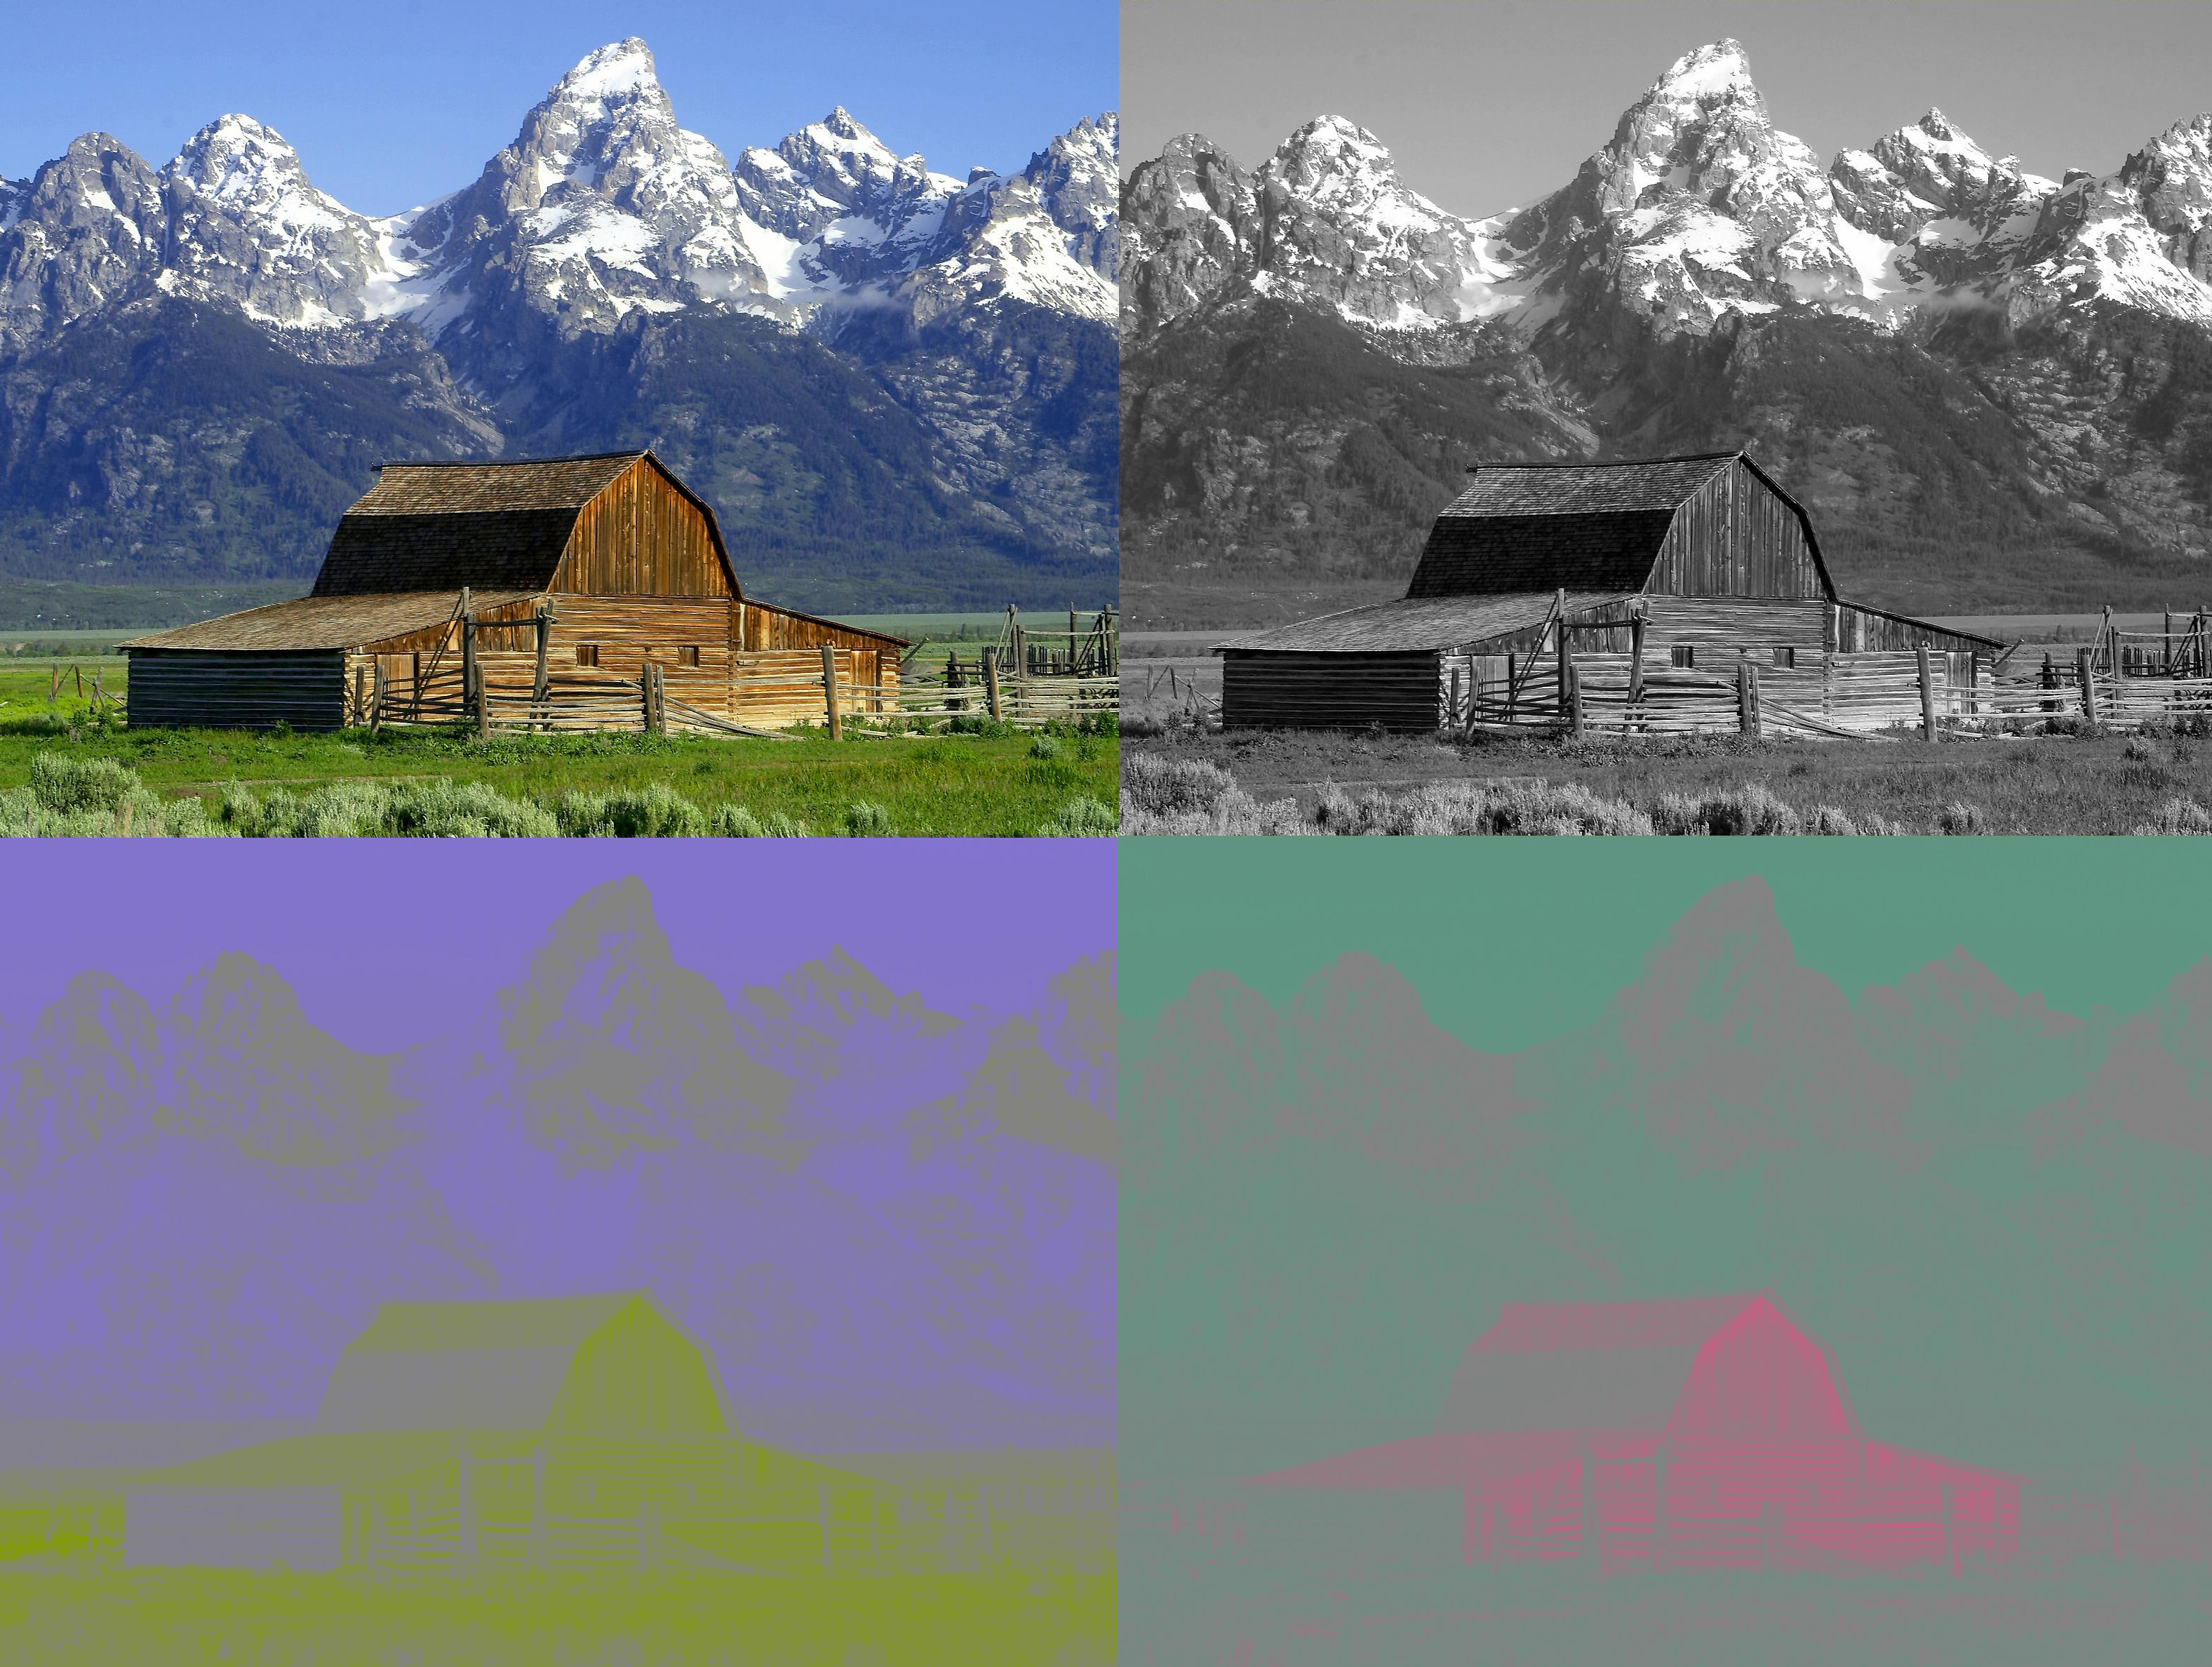
\includegraphics[height=0.4\textheight]{images/Barns_grand_tetons_YCbCr_separation_quad.jpg}}
%popis obrazku
\caption[Example of YCbCr color space (Public domain)]{Example of YCbCr color space. 
Left upper corner is an original image,
right upper corner --- Y channel (grayscale version of image),
left lower --- Cb channel,
right lower --- Cr channel.}
%id obrazku, pomocou ktoreho sa budeme na obrazok odvolavat
\label{img:YCbCr}
\end{figure}

\subsubsection{Downsampling}

Human eye is more sensitive to small changes of brightness rather 
than small changes in the hue and color saturation. Using that fact, 
we can use less space to represent Cr and Cb channels with almost no visible change
to an image. 

There are many options, but one of the most used is to use 4 bits instead of 8
to represent Cr and Cb and 8 bits to represent Y channel (so Y channel is left unchanged).

\subsubsection{Splitting into blocks}

Each channel is divided into $8 \times 8$ bytes long blocks and 
then processed separately. If channel is not exact multiple of block size,
then incomplete blocks are filled with fake values (there are several
methods to construct them, but details are irrelevant for our purposes. 
For further information, you may read \TODO source).

\subsubsection{Discrete cosine transformation}

\begin{comment}
Each block could be seen as finite integer sequence.
This sequence can be seen as values of some function $f$ 
in predefined points $x_1$, $x_2$, \ldots, $x_{64}$.

Discrete cosine transformation is a way of representing this
function as a linear combination of sinusoids (so called \textit{basis functions}) 
based on values of $f(x_1)$, $f(x_2)$, \ldots, $f(x_{64})$. Coefficients of this
linear combinations are called \textit{the DCT coefficients} and
are stored instead of original values, because the original 
values can be later evaluated from them. Figure \ref{img:DCTbf} shows the basis functions.

\end{comment}

Dicsrete cosine transformation is a way of representing block of pixels as 
a linear combination of so called \textit{basis functions}, showed on figure \ref{img:DCTbf},
so we can store coefficients of linear combination instead of the original values.

% source: \url{https://en.wikipedia.org/wiki/File:Dctjpeg.png}
\begin{figure}
%vlozenie samotneho obrazku vycentrovaneho a vhodnej velkosti
%obrazok je v subore images/cervik.png
\centerline{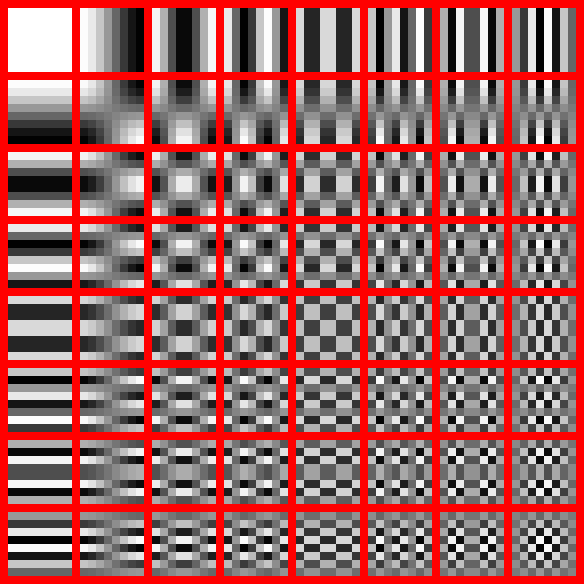
\includegraphics[width=0.5\textwidth]{images/Dctjpeg.png}}
%popis obrazku
\caption[DCT basis functions (Public domain)]{DCT basis functions.}
%id obrazku, pomocou ktoreho sa budeme na obrazok odvolavat
\label{img:DCTbf}
\end{figure}



\subsubsection{Rounding of DCT coefficients}

Here we use two facts. First, DCT basis functions varies from simple
to very complex. Second, human eye is less capable to distinguish such
fine local changes. Therefore, we can represent coefficients of complex
basis functions with less definition (in other words, quantize them).

The level of quantization is defined by demanded quality ratio.

The most fine quailty $Q=100\%$ let all coefficients be rounded to whole numbers,
so it still would be lossy operation.

\subsubsection{Lossless compression of DCT coefficients}

Another interesting property of DCT is that the coefficients
of last basis functions are often very small (because DCT "tries"
to express image with the first sinusoids). Therefore, after
quantisation process many of DCT coefficients could be zero.

The coefficients in each block are ordered in so called \emph{zigzag}
order (by the diagonals from the left upper corner of the block) and
then encoded by Huffman encoding \TODO the ending.

\TODO add an image of the zigzag order


As could be expected, long sequences of zeros could be efficiently
compressed, and therefore significant compress ratio could be achieved.


\section{How to hide information in JPEG?}
\label{sec:how-to-hide-information}

\textit{This section is based on article \cite{liu2008high}.}


An image encoded in JPEG format could be seen as a bunch of (quantized)
DCT coefficients, which are just regular integer numbers. One of the
most natural ideas is to change least significant bits (LSB) of these
numbers to store our message, as these changes are mostly invisible
for human eye and the message can be extracted without knowledge of
the original image.

Problems with direct application of this method is that coefficients with values
$0$ or $1$ would be changed drastically and it would create great disproportion
in amount of zeros and ones.

Modern algorithms try to fight with statistical approach by devising ways to
keep intact various statistical properties of resulting numbers. 

\subsection{JSteg library (direct LSB)}

This library embed secret message in least significant bits of DCT coefficients sequentially.

This approach was quite common for a period of time (there were even algorithms that performed such embedding
in lossless images), but in year 1999 Westfeld and Pfitzmann came up with a so called \textit{chi-square attack}.

\subsection{Chi-square attack}

As you can see in the original paper \cite{westfeld1999attacks}, 
this attack was initially pointed against algorithms with lossless cover images, 
but this approach can be applied for JPEG images too.

Westfeld and Pfitzmann pointed out, that relative amount of values of the DCT coefficients (or pixels in the original paper), 
which differ only in their LSB (so called \textit{paired values}, or \textit{PoV}), is mostly very far from equal 
(i.e. there it is more probable that there would be $1000$ coefficients with value $30$ and $4000$ coefficients with value $31$
than that there would $2500$ of each).

Assuming that 0 and 1 bits are distributed uniformly in the secret message 
(which is usually the case for compressed and/or encrypted message), relative
amount of PoVs becomes equal. And assuming sequential writing in DCT coefficients, one can test
whether paired values show such behaviour. The corresponding statistics has chi-square
distribution, from which this attack got its name.

Let there be $M$ different PoV in the image (e.g. one pair could be $20$-$21$). Let $N_{k, 0}$ ($k \in \{ 1, \ldots, M\}$)
denote the amount of coefficients of $k$-th PoV with $0$ in the least significant bit. Analogically,
$N_{k, 1}$ would denote the amount of coefficients with $1$ in the least significant bit. 
Let denote $N_k := N_{k, 0} + N_{k, 1}$. It is important that the LSB steganography does not change
any of $N_k$.
 
Let our null hypothesis be that an encrypted message (with uniform distribution of $0$ and $1$) 
was embedded into these coefficients (and alternative 
hypothesis would be the opposite sentence). Assuming the null hypothesis, we can see $N_{k, 0}$ as a random
variable following binomical distribution with $n = N_k$ and $p = \frac{1}{2}$, i.e.
$$N_{k, 0} \sim Bin\left(N_k, \frac{1}{2}\right)$$
This distribution can be approximated with normal distribution, i.e.
$$N_{k, 0} \overset{\cdot}{\sim} N\left(\frac{N_k}{2}, \frac{N_k}{4}\right)$$
We can then normalize that variable to $N(0, 1)$ distribution, i.e.
$$ \tilde{N}_{k, 0} := \frac{N_{k, 0} - \frac{N_k}{2}}{\sqrt{\frac{N_k}{4}}}  \overset{\cdot}{\sim} N( 0, 1)$$

Then the sum of squares of such random variables $\tilde{N}_{k, 0}$ would approxiamtely follow the $\chi^2$ distribution with $M-1$
degrees of freedom (we subract one because the sum of all variables is fixed), i.e.
$$\sum_{k = 1}^{M} \tilde{N}^{2}_{k, 0} \overset{\cdot}{\sim} \chi^2_{M-1}$$

We can simplify the expression a bit to get the final statistics: 
$$\sum_{k = 1}^{M} \tilde{N}^{2}_{k, 0} = 
\sum_{k = 1}^{M} \left(  \frac{N_{k, 0} - \frac{N_k}{2}}{\sqrt{\frac{N_k}{4}}}  \right)^2 =
\sum_{k = 1}^{M} \frac{\left(N_{k, 0} - \frac{N_k}{2}\right)^2}{\frac{N_k}{4}} = 
\sum_{k = 1}^{M} \frac{\left(2 N_{k, 0} - N_k\right)^2}{N_k}
=: T
$$ 

Now we can construct a test for our hypothesis. We can do it, for example, by evaluating
the $(1 - \alpha)\%$ confidence interval ($\alpha$ is usually chosen as $5\%$) for $\chi^2$ distribution, which is equal to 
$\left( \chi^2_{M-1}\left(\frac{\alpha}{2}\right), \chi^2_{M-1}\left(1 - \frac{\alpha}{2}\right) \right)$, where $\chi^2_{M-1}(x)$ 
is a $x$-th quantile of this distribution.
(e.g. for $\alpha = 5\%$
and $M=100$ this interval is equal to $(73.36108, 128.422)$). 

The test then work in following way: if evaluated $T$ statistics is 
out of the confidence interval, then the null hypothesis is rejected, i.e. it is unprobable that there is a hidden message. 

This attack could be extended to random writing (i.e. that DCT coefficients to be used
are chosen randomly) by using shifting windows, so we can speak about \textit{extended chi-square attack}. 
This approach is decribed in the paper \cite{provos2001detecting}.

\subsection{F5 algorithm}

In order to defend against chi-square attack, Westfield and Pfitzmann proposed to use 
subtraction operation to match the secret bit inspite of the replacing the last bit. In this way,
the PoVs (decribed in previous subsection) won't be so drastically changed. This approach was applied
in Westfeld's algorithm F5 (decribed in paper \cite{steganalysis2001f5}).

The algorithm is a bit complex, and so it wa originally described as a series of algorithms (thus the number $5$)
with gradual removal of the flaws.

F3 algorithm decreases the absolute value of the coefficients to match the secret bits inspite of their replacement, 
thus being resistant against chi-square attack. Because of this approach, it skips zero coefficients. The problem is
that if the original coefficient has the absolute value $1$ and the secret bit is $0$, then after the embedding
the coefficient would be $0$. The receiver cannot distinguish between unused and decremented zeros, so algorithm
has to embed this bit in the next coefficient available.

This approach leads to two problems: F3 created more zeros than ones in the LSB of coefficients, creating the peculiar
statistically detectable histogram, and that the original JPEG coefficients contain more odd than even values, and so
the \emph{unchanged} part of a message contains more ones than zeros in LSBs.

F4 solves these problems by inverting the meaning of negative coefficients, so that odd negative coefficient means $0$
and even negative means $1$.

F4 and F3 both suffer from sequential using of the DCT coefficients. F5 removes this weakness by choosing the coefficients
in a random way (based on a stegonagraphic key). Additionally, F5 uses so called \emph{matrix encoding} to increase effectiveness
of embedding ratio (bits of information per modified coefficient).

F5 algorithm is currently used in many steganographic Android apps, mainly because of its open Java implementation. However, this
algorithm can be successfully attacked with so called \emph{S attack}.


\subsection{S-family attacks}

S-family is a general framework of attacks. The basic idea is that one can find (empirically) some specific macroscopic 
characteristic $S(p)$ of images, which changes predictably (e.g. monotonically increases) 
with the length of the embedded secret message~$p$ (i.e. this function is specific for every algorithm). 
One can then estimate critical of this function $S$ (i.e. $S(0)$ --- characteristic for an empty embedded message and
$S(max)$ --- for the maximal possible message length). Then he has to sovle the equation $S(q) = x$, where $x$ is a given
image with embedded message and $q$ is an estimation of this embedded message. $S(max)$ can be obtained by embedding of
maximum possible message to obtained cover image (so it will rewrite the original hidden message), and $S(0)$ can be obtained
by cropping the cover image and recompressing with the original quantization table. You can read more about general structure
here \cite{fridrich2002attacking}.

For F5 algorithm, the $S$ was chosen as ''blockiness'' of the image. The process is decribed in \cite{fridrich2002steganalysis}.

\subsection{Complementary embedding algorithm (CE)}

This algorithms was designed to be resistant against both S and chi-square attacks designed for F5 and JSteg.

Because it's the algorithm we had used in our application, 
we've decided to put the description of this algorithm in chapter \ref{chap:theory}
along with the decsriptions of other used algorithms (you can find it in the subsection
\ref{ssec:ce}).

\subsection{Attacks based on Benford's law}

This approach was described in \cite{andriotis2013two} and \cite{andriotis2013jpeg}.

Benford's law states that in a random set of integer numbers the most significant digit would
with the highest probability be $1$, second highest would be $2$, and so on. Formally, if we denote $x$
as the most significant digit, the law could be written as this:
$$P(x = 1) > P(x = 2) > P(x = 3) > \ldots > P(x = 9),$$
where $P(x = i)$ is probability that the most significant digit is equal to $i$.

This law was given a numerical form:
$$p(n) = \log_{10}\left(n + \frac{1}{n}\right) ~\left(i \in \left\{ 1, \ldots , 9 \right\}\right),$$
where $p(n)$ denotes the probability that the most significant digit is equal to $n$.

This law is being used to detect elections riggings (usually authors use the Benford's law modified to 
describe second digit distribution). You can read more in these papers
\cite{mebane2006election, roukema2009benford, deckert2011benford}.

Fu et al. in \cite{fu2007generalized} studied distribution of quantized DCT coefficients (specifically, the distribution of first digits)
and proposed a Benford-like distribution (which they called \emph{general Benford's law}):
$$p(n) = N \cdot \log_{10}\left(n + \frac{1}{s + n^q}\right) ~\left(i \in \left\{ 1, \ldots , 9 \right\}\right), $$
where $N$, $s$ and $q$ are parameters dependent on used quality ratio (note that the original form can be obtained when
$N = 1$, $s = 0$ and $q = 1$).

The algotithm is easy: we need a precomputed table of paremeters for each quality ratio. Then we extract DCT coefficients
from a cover image, compare their first digits' distribution, compare to the expected distribution and decide whether to
declare the image as "suspicious". Details can be found in the original paper \cite{andriotis2013two}.

This method is very interesting because of seeming effectiveness: authors claim they can detect even a 1kB of embedded data
in the image of size $800 \times 600$.

\subsection{Attacks using higher order statistics}

While many steganographic algorithms aim to preserve first-order statistics of cover images
(i.e. histograms of coefficients), higher order statistics (variance, skewness and kurtosis)
appear to be harder to preserve.

Algorithm, proposed by Siwei Lyu and Hany Farid in \cite{lyu2002detecting}, expoits this fact.
Firstly, it decomposes a cover image by using separable quadrature mirror filters (QMFs) \cite{vaidyanathan1987quadrature}.
This filter essentially separates the image into several subimages by their frequencies (frequencies are meant as patterns,
where more complex structures are referred to as \emph{higher frequencies}).
Secondly, it evaluates corresponding statistics (mean value, variance, skewness and kurtosis, mentioned earlier).
Thirdly, it obtains additional information from errors of optimal linear prediticion of coefficients magnitude.
Fourthly, it evaluates the same 4 statistics of these data.

This process is applied on a training set of images, both with hidden messages and without. Then algorithm
applies a general classification method (originally authors had used Fisher linear discrimination analysis \cite{welling2005fisher}, now
they use support vector machines (SVM) \cite{vapnik2013nature}). After training, the model is ready to detect images with hidden messages.

Main drawback is a need of a representative training set. 

\subsection{Algorithm Pm1 based on genetic algorithms (GA)}


\TODO add Pm1 using genetic algorithms

\subsection{Attacks based on DCT coefficients probability distributions}
\TODO short mentioning about modern approaches

\section{Present state of free and/or open-source programs}
In this section we will show common mistakes of available applications for Android.

We've reviewed several free applications in Google Play:
\begin{itemize}
    \item \app{Steganography}{Jan Meznik}{https://play.google.com/store/apps/details?id=com.meznik.Steganography}
    \item \app{Steganography Master}{Dino Trnka}{https://play.google.com/store/apps/details?id=com.dinaga.photosecret}
    \item \app{NiaStego}{Newidget Dev}{https://play.google.com/store/apps/details?id=dev.nia.niastego}
    \item \app{Pocket Stego}{Talixa Software}{https://play.google.com/store/apps/details?id=com.talixa.pocketstego} 
    \item \app{Hidden Secrets}{Shweta Gupta}{https://play.google.com/store/apps/details?id=stego.lsb.hiddensecret}
    \item \app{Secret Messages CryptApp}{FlyJam}{https://play.google.com/store/apps/details?id=flyjam.CryptApp}
    \item \app{Stego Message}{Evgeny Shishkin}{https://play.google.com/store/apps/details?id=com.shishkin.steganographie}
    \item \app{VipSecret}{icokocev}{https://play.google.com/store/apps/details?id=com.vipcontest.vsecret}
    \item \app{PtBox FREE}{TROTTA Gianpaolo Francesco}{https://play.google.com/store/apps/details?id=gftrotta.dpatruno.ptboxfree}
    \item \app{Steganosaurus}{Studio Mastodonte}{https://play.google.com/store/apps/details?id=app.steganosaurus}
    \item \app{Stegos}{Panacom, s.r.o.}{https://play.google.com/store/apps/details?id=sk.panacom.stegos}
    \item \app{Stegosaurus}{abeatte}{https://play.google.com/store/apps/details?id=com.artbeatte.stegosaurus}
    \item \app{Stegais}{Roman Chinkais}{https://play.google.com/store/apps/details?id=com.romancinkais.stegais}
    \item \app{Secret Tidings}{Phoebit}{https://play.google.com/store/apps/details?id=com.phoebit.secrettidings}
    \item \app{Da Vinci Secret Image}{RADJAB}{https://play.google.com/store/apps/details?id=jubatus.android.davinci}
    \item \app{PassLok}{Francisco Ruiz}{https://play.google.com/store/apps/details?id=com.fruiz500.passlok}
    \item \app{StegoLite}{Bearded Man}{https://play.google.com/store/apps/details?id=jepaweb.stegasaurus}
    \item \app{Kryfto}{Batsakidis Athanasios}{https://play.google.com/store/apps/details?id=it.kryfto}
    \item \app{CrypTego}{QitVision}{https://play.google.com/store/apps/details?id=com.qitvision.cryptego}
    \item \app{PixelKnot}{The Guardian Project}{https://play.google.com/store/apps/details?id=info.guardianproject.pixelknot}
\end{itemize} 

\subsection{Common mistakes}

\subsubsection{Closed implementation}
Steganography and cryptography could be very complicated to implement correctly, so applications with
no open code should always be treated with a grain of salt.

\subsubsection{Unknown steganographic and/or cryptographic algorithms}
Digital image steganography is a very young field and new algorithms and attacks appear every year.
In this context it is highly unrecommended to use old applications or applications with no such 
specification.

\subsubsection{No limitation for message length}
As there are blind steganalytic methods, which does not depend on used steganographic algorithm 
(such as using higher order statistics or Benford's law, described in section \ref{sec:how-to-hide-information}),
it is unrecommended to send large messages.

\subsubsection{Low upper limit for a key}
Some apps (e.g. \emph{Steganography} by Jan Meznik) has upper limit for a key set as $8$ symbols, which is considered low
by any standard.

\subsubsection{Lossless images used as carrier}
It is highly unrecommended to use lossless image formats as cover images. We've discussed this matter in section \ref{sec:image-steganography}
(this is a case for application \emph{NiaStego}).

\subsubsection{No support of non-latin symbols}
Some applications (e.g. \emph{Pocket Stego}) has only ASCII support.

\subsubsection{Predefined cover images and possibility to use same images repeatedly}
It is highly unrecommended to use the same image twice as a carrier, let alone having 
a predefined set of images (this is a case for application \emph{VipSecret}).

\subsubsection{Steganographic algorithm is not key-dependant}
Keyless algorithms are very vulnerable to attacks (it would suffice in that case
to use the original application to detect hidden message).

\subsubsection{No encryption nor compression}
Most of steganographic algorithm work under the assumption that a message has uniform distribution
of $0$ and $1$ (which is a case for encrypted message).
